\documentclass[a4paper]{article}

%% Language and font encodings
\usepackage[english]{babel}
\usepackage[utf8x]{inputenc}
\usepackage[T1]{fontenc}
\usepackage[normalem]{ulem}
\usepackage{minted}
%% Sets page size and margins
\usepackage[a4paper,top=3cm,bottom=2cm,left=3cm,right=3cm,marginparwidth=1.75cm]{geometry}

%% Useful packages
\usepackage{amsmath}
\usepackage{color}
\usepackage{graphicx}
\usepackage{wrapfig}
\usepackage[colorinlistoftodos]{todonotes}
\usepackage[colorlinks=true, allcolors=blue]{hyperref}
\usepackage{listings}

\title{PHYS 370\\
Computational Physics\\}
\author{Jacob William Connelly\\
David Jedynak\\
Nick Zahler}
\date{March 07, 2018}
\begin{document}
\maketitle

\section{Abstract}
\paragraph{}
The semiconductor device is where electrical engineering meets quantum physics. By understanding the crystalline lattice structure of molecules and how charge carriers move through them, the ability to manipulate them was derived. 'Doping', the deliberate process of adding impurities into a structure, is the base theory behind the modern semiconductor. By placing two (differently) doped structures next to one another, a junction is created; this meeting of doped crystalline structures is the science behind all modern day electronics, including transistors and integrated circuits. Our experiment will seek to simulate with 3D visualizations based on C code the most basic of the semiconductor structures, the diode; a device that, when doped, only allows current to flow unidirectionally; this paper is the documentation of that experiment.

\section{Introduction}
\paragraph{}
To work through this problem we first needed to understand, in depth, the inner workings of the diode and how electricity moves through it, and why. This process was made relatively easy, since all group members have a background in electrical engineering. The trick was in figuring out how to take our knowledge of the physical chemistry of a diode, the understanding of its electrical properties, and translate that into a computer simulation. 
	The diode simulation takes the form of a plane with various fields placed along its length. For easy visualization, the different fields are denoted by lines that stretch across the plane. When the program runs with a voltage source applied in the 'proper' orientation, current will flow across the diode. However, as would happen in reality, if the voltage source is 'backwards' (or, in effect, the diode turned the other direction), current flow stops. \\
    
   

\section{Theory}
\paragraph{}
Semiconductors are unique in the electrical world in that they are able to both conduct and repel electric current. They are made of material that has an electrical conductivity between strong electric conductors, such as gold or copper, and insulators, such as rubber or plastic. The most commonly used element for semiconductor devices is silicon, a metalloid in the periodic table. Pure silicon has no free electrons, which is why the element is doped to give it enhanced electro-conductive properties. The doping process includes introducing impurities into the silicone crystal, as can be seen in Figure 1.

\begin{figure}[H]
\centering
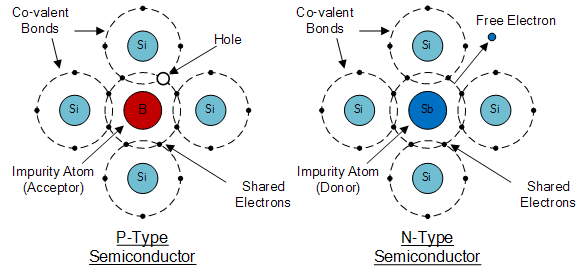
\includegraphics[scale=0.8]{doping.PNG}
\caption{\label{fig} Diagram of doping process}
\end{figure}

As noted in the figure above, N-type doping adds an impurity to the silicone structure that introduces free electrons, while P-type introduces vacant positions, or 'holes', for free electrons to fill. 

A diode is the physical object that puts this doping into practice at its most basic level. At the junction where P-type and N-type meet is where things get interesting. The extra electrons from the N-type transition over to the P-side, which gives the P-side a slightly negative charge. Simultaneously, since the electrons have moved out of the N-type region, that area gets a slightly positive charge. The electric field that results from this is known as the depletion region, which can be seen below.

\begin{figure}[H]
\centering
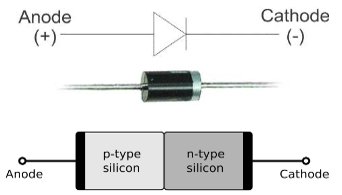
\includegraphics[scale=0.75]{Diodes2.PNG}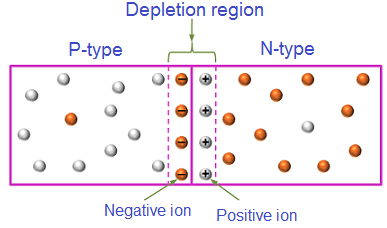
\includegraphics[scale=0.6]{Depletion.PNG}
\caption{\label{fig} Physical diode and representations (left), Depletion region (right)}
\end{figure}

The depletion region is the basis of the barrier that stops electron flow. Applying current to the diode "backwards" results in what is known as reverse biasing, in which the depletion zone widens as power source attracts both electrons and holes. However, when connected the other way, and if an electron has enough energy, it can overcome the barrier potential and cross the depletion region. Negative electrons are pushed away by negative terminal, and "fall into the holes", depleted of energy. The electrons behind it cross the barrier and occupy the next line of holes, and so on, until the holes are full, and electricity passes through the diode. This result is the one-way flow of electricity. 

In an ideal world with perfect conditions, the graph of Voltage vs Current (V vs I) should be zero at all points from negative infinity to 0V, then instantaneously spike along the y-axis at V>=0. In effect, the diode would be treated as nothing but a wire. In reality there are physical limitations on the chemical structure of silicone, which is why we need to reach a certain voltage potential before the barrier potential can be crossed. For silicone diodes, this happens at right around 0.7V. In the other direction, if a strong enough negative voltage is applied to the diode, it will eventually overpower the depletion zone and current will flow. This phenomena is known as 'breakdown', but only happens at voltages stronger than -50V, and will not be simulated in our experiment. The voltage vs current graphs of ideal vs real diodes is shown below. 

\begin{figure}[H]
\centering
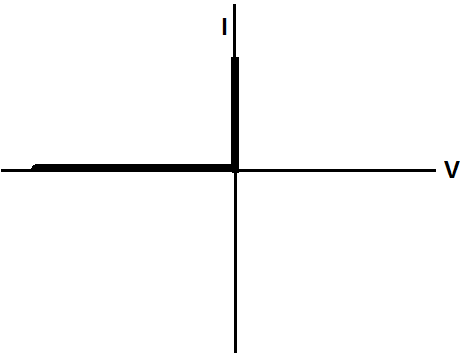
\includegraphics[scale=0.6]{08.png}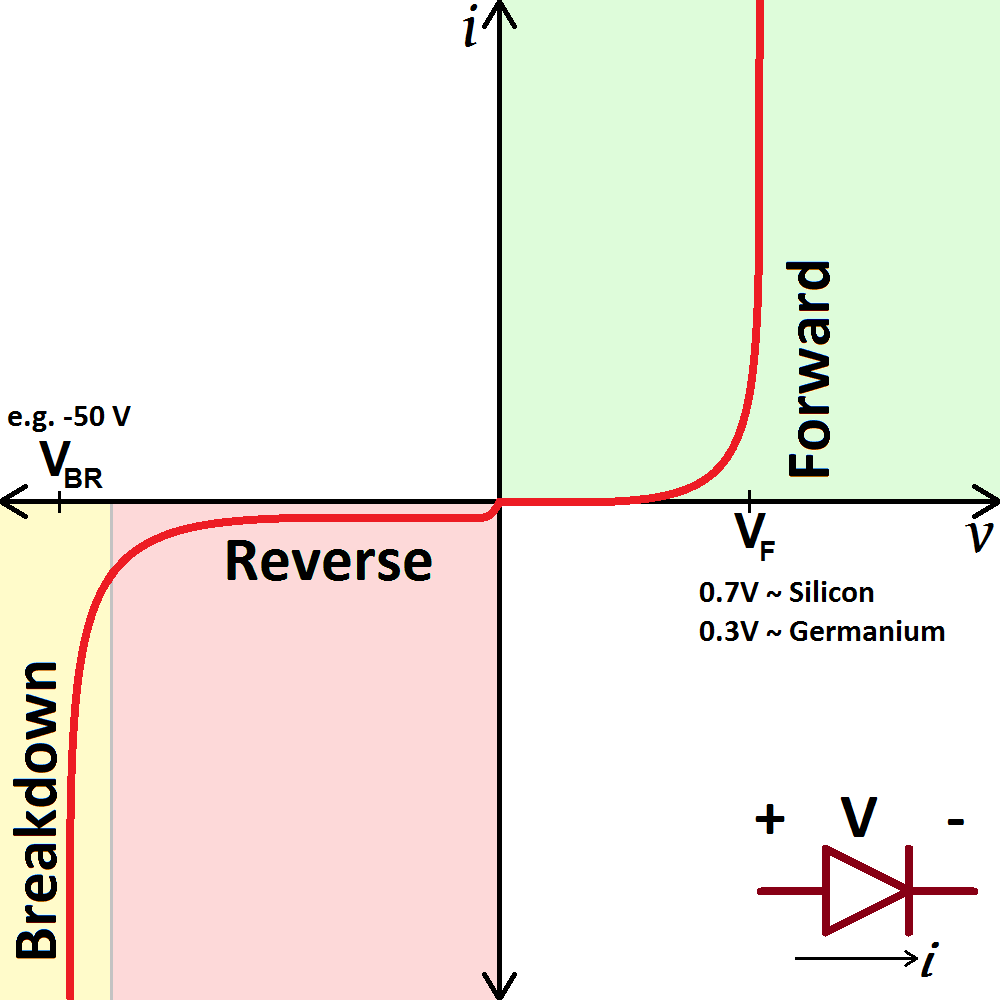
\includegraphics[scale=0.23]{06.png}
\caption{\label{fig} Ideal V vs I graph (left), Real V vs I graph (right)}
\end{figure}

\section{Procedure}
\paragraph{}

\begin{enumerate}
\item Open terminal and launch the Diode program with the following command
\begin{minted}{bash}
  $ ./Diode_Exec
\end{minted}
\item Click init, measure, Measurements and Diode. All of these should bring up a separate window. Arrange these on your desktop so you can see all of them.
\item leave other settings to defaults
\item in the Measurements window, click Average Current to open a graph of current over time. This should have a dynamic graph once cont is set to on.
\item {\sout{ in the measure window, set T = 2, click "Set T"}}
\item In the Diode window, click SetVoltageSource to initialize the voltage.
\item in the main window, set cont to on
\item {\sout{ immediately click set T to keep the T at 2}}
\item {\sout{ repeat step 8 until the T (temperature) on the Measurements graph settles to 2+-0.1.}}
\item {\sout{ click the cont button in the main window to stop the simulation}}
\item {\sout{ record the values of P (pressure) Pnid (ideal pressure) and T (temperature) to be plotted later}}
\item {\sout{ change the value of rho in the measure window to 0.4 and click "set rho"}}
\item {\sout{ click cont in the main window to resume the simulation}}
\item {\sout{ repeat steps 6 to 13 with different rho values of [0.5, 0.6, 0.7 ,0.8 ,0.9 ,1.0 ,1.1 ,1.2 ,1.3 ,1.4 ]}}
\item {\sout{ plot the values T, P, Pnid vs rho to see how these values changed with respect to changing density}}
\item {\sout{ repeat steps 5 to 15 with a T value of 0.05 and rho values of [0.5 ,0.4     ,0.3   ,0.2   ,0.15   ,0.1    ,0.08   ,0.06   ,.04   ,0.02     ,   0.01]}}
\end{enumerate}
\section{Algorithms and Code}
\paragraph{}


\section{Results}
\paragraph{}
\begin{enumerate}
\item Results for Forward-Biasing\\
voltage sweep, -5V - 5V
increments of 1v
\item Results for Reverse-Biasing
voltage sweep -10V - 150V
increments of 10v
\end{enumerate}
 \textcolor{red}{Analyse the data your code is generating. 
    \\Do the results agree with your hypothesis? \\
    How are the results different from your expectations?\\
    What does that tell you about your project?}\\
\textcolor{red}{INSERT SCREENSHOTS OF CODE WORKING, GRAPHS, ETC}



\section{Conclusion}
\paragraph{}
\textcolor{red}{WHAT UNEXPECTED DIFFICULTIES DID YOU ENCOUNTER? HOW DID YOU ADDRESS THEM?}

\section{Individual Contribution}
\paragraph{}
 \textcolor{red}{ADD BIT ABOUT HOW WORK WAS DIVIDED AMONG GROUP}\\
 \textcolor{red}{Each group member will fill out the section next to their name.\\
Jacob Connelly:\\
David Jedynak:\\
Nick Zahler:\\}

\section{Code for Diode Simulation}
\paragraph{}
\textcolor{red}{PUT CODE HERE}
\begin{lstlisting}
/*CODE*/

\end{lstlisting}
\section{References}
\paragraph{}
https://www.ndsu.edu/pubweb/~carswagn/LectureNotes/370/index.html
\end{document}


++++++++++++

